\documentclass[11pt]{article}


\usepackage[sort]{natbib}
\usepackage{bm,amsmath,bbm,amsfonts,nicefrac,latexsym,amsmath,amsfonts,amsbsy,amscd,amsxtra,amsgen,amsopn,bbm,amsthm,amssymb,graphicx}
\usepackage{fancyhdr}
\usepackage{caption}
\usepackage{subcaption}
\usepackage{color}
\usepackage[margin=1.0in]{geometry}


\title{Information content for observations of forest carbon stocks and fluxes when assimilated with the DALEC carbon balance model}
%\date{\normalsize{3$^{\text{rd}}$ June 2014, \ Room 1L36}}
\author{\normalsize{E. Pinnington}}


\newtheorem{theorem}{Theorem}[section]
\newtheorem*{defn}{Definition}

	
\begin{document}

\maketitle

\section{Introduction}%%%%%%%%%%%%%%%%%%%%%%

A large amount of data is currently being gathered that is relevant to the carbon balance of forests, with much of this data coming from Eddy covariance flux towers \cite{baldocchi2008turner, baldocchi2001fluxnet, running1999global, valentini2000respiration}. Attempts are also being made to combine this data with models of forest carbon stocks and fluxes, such as the Data Assimilation Linked Ecosystem Carbon model (DALEC), in a data assimilation scheme \cite{williams2005improved, fox2009reflex}. Currently, however, there are limitations with such schemes as there is a lack of understanding about the additional information provided by different observations. Better understanding of the information content of carbon balance observations will help inform measurement campaigns of when and which observations to take in order to gain the most possible information about the system. In this report we will look at different information content measures which have been used in meteorological data assimilation \cite{rodgers2000inverse, fisher2003estimation, sandu2012practical} and apply these to carbon balance observations assimilated with DALEC. Although we use DALEC in this report the results will be similar for other carbon balance models which use similar driving data and equations. We begin by introducing the DALEC model which will initially be used to look at the information content in different observations.

\section{The DALEC Model}%%%%%%%%%%%%%%%%%%%%%%

The DALEC model is a simple process-based model describing the carbon balance of an evergreen forest ecosystem \cite{williams2005improved}. The model is constructed of five carbon pools (foliage ($C_f$), fine roots ($C_r$), woody stems and coarse roots ($C_w$), fresh leaf and fine root litter ($C_l$) and soil organic matter and coarse woody debris ($C_s$)) linked via fluxes. The gross primary production function ($GPP$) uses meteorological driving data and the site's leaf area index (a function of $C_f$) to calculate the total amount of carbon to be allocated at a daily time step.   

\begin{figure}[h]
    \centering
    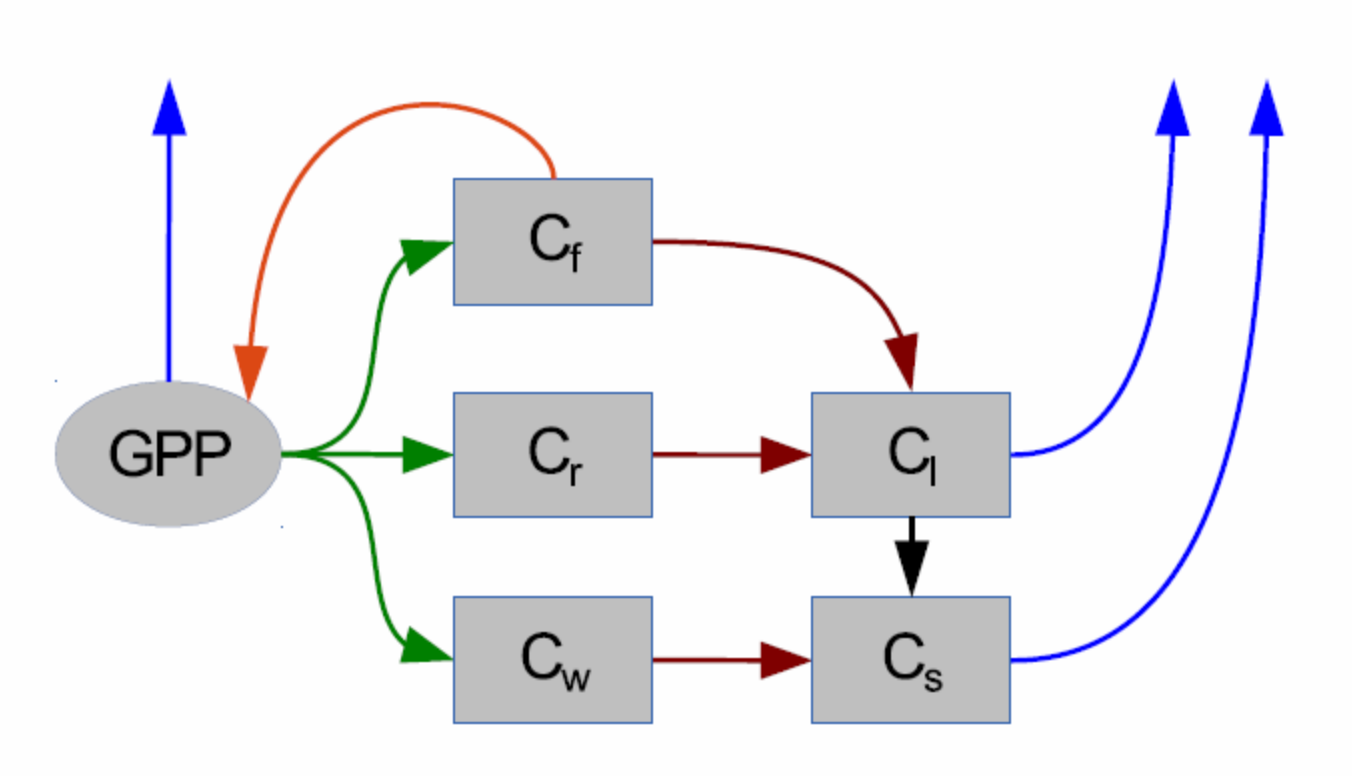
\includegraphics[width=0.5\textwidth]{DALECpic.png}
    \caption{Representation of the carbon fluxes in the DALEC carbon balance model. Green arrows represent C allocation, dark red and black arrows represent litterfall and decomposition fluxes, blue arrows represent respiration fluxes and the light red arrow represents the feedback of foliar carbon to the $GPP$ function. \cite{delahaies2013regularization}}
    \label{fig:DALEC_mod}
\end{figure}

The model equations for the carbon pools at day $t+1$ are as follows:

\begin{align}
C_f(t+1)&=(1-p_5)C_f(t)+p_3(1-p_2)GPP(C_f(t),\phi), \label{dalec1}
\\C_r(t+1)&=(1-p_7)C_r(t)+p_4(1-p_3)(1-p_2)GPP(C_f(t),\phi), 
\\C_w(t+1)&=(1-p_6)C_w(t)+(1-p_4)(1-p_3)(1-p_2)GPP(C_f(t),\phi), 
\\C_l(t+1)&=(1-(p_1+p_8)T(t))C_l(t)+p_5C_f(t)+p_7C_r(t), 
\\C_s(t+1)&=(1-p_9T(t))C_s+p_6C_w(t)+p_1T(t)C_l(t), \label{dalec5}
\end{align}

where $T(t)=\frac{1}{2}exp(p_{10}T_m(t))$, $T_m$ is daily mean temperature, $p_1,\ldots,p_{10}$ are rate parameters and $\phi$ represents the meteorological driving data used in the $GPP$ function. The full details of this version of DALEC can be found in \cite{williams2005improved}, it is paramterized for data from a young pine stand in Ponderossa, Oregon, we include values of the model parameters and the equations used to calculate $GPP$ in the appendix. We now see how DALEC can be implemented in a four-dimensional variational data assimilation (4D-Var) framework.

\subsection{DALEC in a variational assimilation framework}\label{4dvardalec}%%%%%%%%%%%%%%%%%%%%%% 

In 4D-Var we aim to maximise the probabiliy of our initial state $\textbf{x}_0$ (for DALEC our state $\textbf{x}_0$ corresponds to the initial values of the five carbon pools,  $\textbf{x}_0 = (C_f(t_0), C_r(t_0), C_w(t_0), C_l(t_0), C_s(t_0))^T$) given a set of observations $\textbf{y}$, $P(\textbf{x}_0|\textbf{y})$, over some time window, $N$. We do this by minimising a cost function $J(\textbf{x})$ derived from Baye's Theorem \cite{lewis2006dynamic}. The cost function is given as,

\begin{equation}
J(\textbf{x}_0) = \frac{1}{2}(\textbf{x}_0-\textbf{x}_b)^{T}\textbf{B}^{-1}(\textbf{x}_0-\textbf{x}_b)+\frac{1}{2}\sum_{i=0}^{N}(\textbf{y}_i-h_i(\textbf{x}_i))^{T}\textbf{R}_{i}^{-1}(\textbf{y}_i-h_i(\textbf{x}_i)),
\end{equation}•
where $\textbf{x}_b$ is our background and acts as our initial guess to our state $\textbf{x}_0$, $\textbf{B}$ is the background error covariance matrix and quantifies our knowledge of the error in our background, $h_i$ is our observation operator at time $t_i$ and maps our state vector evolved by our nonlinear model ($\textbf{x}_i$) to the observations at this time $\textbf{y}_i$ and $\textbf{R}_i$ is the observation error covariance matrix and represents our knowledge of the uncertainty in the observations. The state that minimises the cost function is called the analysis and is denoted as $\textbf{x}_a$, this state is found using a minimisation routine that takes the cost function, our initial guess ($\textbf{x}_b$) and also the gradient of the cost function defined as,

\begin{equation}
\nabla J(\textbf{x}_0) = \textbf{B}^{-1}(\textbf{x}_0-\textbf{x}_b)-\sum_{i=0}^{N}\textbf{M}_{i,0}^{T}\textbf{H}_i^{T}\textbf{R}_{i}^{-1}(\textbf{y}_i-h_i(\textbf{x}_i)),
\end{equation}•
where $\textbf{H}_i = \frac{\delta h_i(\textbf{x}_i)}{\delta\textbf{x}_i}$ is our linearized observation operator, $\mathbf{M}_{i,0}=\mathbf{M}_{i-1}\mathbf{M}_{i-2}\cdots\mathbf{M}_0$ is our tangent linear model with $\mathbf{M}_i=\frac{\delta \textbf{m}_i(\textbf{x}_i)}{\delta \textbf{x}_i}$. We can calculate the linearized model for DALEC from equations \ref{dalec1} to \ref{dalec5} as,
\begin{equation}
\mathbf{M}_{i}= 
\begin{pmatrix} 
(1-p_5)+p_3(1-p_2)\zeta_i & 0 & 0 & 0 & 0 \\
p_4(1-p_3)(1-p_2)\zeta_i & (1-p_7) & 0 & 0 & 0 \\
(1-p_4)(1-p_3)(1-p_2)\zeta_i & 0 & (1-p_6) & 0 & 0 \\
p_5 & p_7 & 0 & (1-(p_1+p_8)T_i) & 0 \\
0 & 0 & p_6 & p_1T_i & (1-p_9T_i) \\
\end{pmatrix}, \label{linmod}
\end{equation}
where $\zeta_i = GPP'(C_f(t_i), \phi)$ and $T_{i}=T(t_i)$.

Once we have performed the minimisation of the cost function and determined $\textbf{x}_a$ we can also calculate the analysis error covariance matrix, $\textbf{A}$, to quantify the uncertainty in our new estimate of the state. We can define the analysis error covariance matrix as,
\begin{equation}
\textbf{A} = \big(\mathbf{J}''\big)^{-1} = \big(\mathbf{B}^{-1}+\hat{\mathbf{H}}^{T}\hat{\mathbf{R}}^{-1}\hat{\textbf{H}}\big)^{-1}, \label{Amat}
\end{equation}• 
where $\hat{\mathbf{H}}$ is the matrix of linearized observation operators evolved by the tangent linear model and $\hat{\mathbf{R}}$ is the block diagonal matrix of observation error covariance matrices,
\begin{equation}
\hat{\mathbf{H}}=
\begin{pmatrix}
\mathbf{H}_0 \\
\mathbf{H}_1\mathbf{M}_0\\
\vdots \\
\mathbf{H}_N\mathbf{M}_{N,0}
\end{pmatrix}
\hspace{5mm} \text{and} \hspace{5mm}
\hat{\mathbf{R}}=
\begin{pmatrix}
\mathbf{R}_0 & 0 & 0 & 0 \\
0 & \mathbf{R}_1 & 0 & 0 \\
0 & 0 & \ddots & 0 \\
0 & 0 & 0 & \mathbf{R}_N
\end{pmatrix}.
\end{equation}

\section{Information Content Measures}%%%%%%%%%%%%%%%%%%%%%%

Information content measures are already being used to quantify the different levels of information provided by observations in the development of satellite instruments \cite{stewart2008correlated, engelen2004information} and in operational data assimilation schemes \cite{fisher2003estimation, sandu2012practical}. In these fields two of the more widely used measures are Shannon Information Content (also known as entropy reduction) and the degrees of freedom for signal. We will apply both methods for observations assimilated with DALEC. 

\subsection{Shannon Information Content}%%%%%%%%%%%%%%%%%%%%%%

In DA Shannon Information Content ($SIC$) is a measure of the reduction in entropy given a set of observations. Entropy physically corresponds to the volume in state space taken up by the probability density function ($pdf$) describing the knowledge of the state. When a measurement is made the volume of this $pdf$ decreases, the information content of the measurement is a measure of the factor by which it decreases \cite{rodgers2000inverse}. If $P_b(x)$ is our knowledge of the state before an observation and $P_o(x|y)$ is our knowledge after an observation then we have entropies,
\[
S[P_b(x)] = - \int P_b(x)\text{log}_2[P_b(x)]dx
 \hspace{5mm} \text{and} \hspace{5mm} 
S[P_o(x|y)] = - \int P_o(x|y)\text{log}_2[P_o(x|y)]dx.
\]
The entropy reduction, or $SIC$, due to the observation is then,
\begin{equation} \label{shaic}
SIC =  S[P_b(x)]-S[P_o(x|y)].
\end{equation}
If we assume all $pdfs$ are Gaussian and use the natural logarithm as opposed to $\text{log}_2$ (for algebraic convenience) \cite{rodgers2000inverse} the entropy of a multivariate Gaussian distruibution for a vector $\textbf{x}$ with $n$ elements (before and after observations) can be derived as,
\begin{equation} \label{SB}
 S[P_b(\textbf{x})] = n\text{ln}(2\pi e)^{\frac{1}{2}}+\frac{1}{2}\text{ln}\begin{vmatrix}\bf{B}\end{vmatrix}
\end{equation}
and
\begin{equation} \label{SA}
 S[P_o(\textbf{x}|\textbf{y})] = n\text{ln}(2\pi e)^{\frac{1}{2}}+\frac{1}{2}\text{ln}\begin{vmatrix}\bf{A}\end{vmatrix}
\end{equation}
where $\bf{B}$ is the background error covariance matrix and $\bf{A}$ is the analysis error covariance matrix. Combining equations \ref{shaic}, \ref{SB} and \ref{SA} we can write the $SIC$ as,
\begin{equation}
SIC=\frac{1}{2}\text{ln}\frac{\begin{vmatrix} \bf{B} \end{vmatrix}}{\begin{vmatrix} \bf{A} \end{vmatrix}}.
\end{equation}•
From equation \ref{Amat} we can see the $SIC$ can also be written as,
\begin{equation}
SIC= \frac{1}{2}\text{ln}\begin{vmatrix} \mathbf{B} \end{vmatrix}\begin{vmatrix} \mathbf{J}'' \end{vmatrix}. \label{sic}
\end{equation}•

\subsection{Degrees of Freedom for Signal}%%%%%%%%%%%%%%%%%%%%%%

The degrees of freedom for signal ($DFS$) indicates the number of elements of the state that have been measured by the observations. If we consider a state vector $\textbf{x}$ with $n$ elements (or $n$ degrees of freedom) then the maximum value the $DFS$ could obtain would be $n$, in this case all elements of the state would have been measured. Conversely if $DFS = 0$ then no elements of the state would have been measured by our observations \cite{fowler2011measures}.

We have symmetric positive definite background and analysis error covariance matrices $\bf{B}$ and $\bf{A}$, the eigenvalues of each matrix gives a representation for the uncertainty in the direction of the associated eigenvector, thus by comparing the eigenvalues of both matrices we can determine the reduction in uncertainty given a set of observations \cite{stewart2008correlated}.

In order to do this we take $\mathbf{B}^{\frac{-1}{2}}$ such that $\mathbf{B}^{-1} = \mathbf{B}^{\frac{-1}{2}}\mathbf{B}^{\frac{-1}{2}}$. We now take $\bf{Q}$ to be the orthogonal matrix composed of the eigenvectors of $\mathbf{B}^{\frac{-1}{2}}\mathbf{A}\mathbf{B}^{\frac{-1}{2}}$ we have,
\begin{equation}
\mathbf{Q}^{T}\bigg(\mathbf{B}^{\frac{-1}{2}}\mathbf{A}\mathbf{B}^{\frac{-1}{2}}\bigg)\mathbf{Q} = \bf{\Lambda},
\end{equation}• 
\begin{equation}
\mathbf{Q}^{T}\bigg(\mathbf{B}^{\frac{-1}{2}}\mathbf{B}\mathbf{B}^{\frac{-1}{2}}\bigg)\mathbf{Q} = \mathbf{I}_{n\text{x}n}
\end{equation}•
where $\bf{\Lambda}$ is a diagonal matrix. Each diagonal element of our transformed $\bf{B}$ is equal to one and corresponds to one degree of freedom. The diagonal elements of $\bf{\Lambda}$ correspond to the matrixs eigenvalues and can be interpreted as the relative reduction in variance for each of the $n$ degrees of freedom \cite{sandu2012practical}. We can then define the $DFS$ as,
\begin{equation}
\begin{split}
DFS & = \text{trace}(\mathbf{I}_{n\text{x}n} - \mathbf{\Lambda}) \\
       & = n - \text{trace}(\mathbf{\Lambda}) \\
       & = n - \text{trace}(\mathbf{B}^{\frac{-1}{2}}\mathbf{A}\mathbf{B}^{\frac{-1}{2}}) \\
       & = n - \text{trace}(\mathbf{B}^{-1}\mathbf{A}).
\end{split}
\end{equation}

\section{Shannon Information Content for DALEC}%%%%%%%%%%%%%%%%%%%%%%

We begin by using $SIC$ to understand the information content for different observations when being assimilated with the DALEC model. For these experiments the model is set up as in section \ref{4dvardalec} where the elements of the state vector have standard deviations, $\sigma_{cf,b},\ldots,\sigma_{cs,b}$, respectively. These standard deviations represent the uncertainty in our inital background estimate and are taken as a percentage of the initial carbon pools (these values can be found in the appendix). The background error covariance matrix is then taken as the diagonal matrix of the variances of the carbon pools,
\begin{equation}
\bf{B} = \begin{pmatrix} 
\sigma_{cf,b}^{2} & 0 & 0 & 0 & 0 \\
0 & \sigma_{cr,b}^{2} & 0 & 0 & 0 \\
0 & 0 & \sigma_{cw,b}^{2} & 0 & 0 \\
0 & 0 & 0 & \sigma_{cl,b}^{2} & 0 \\
0 & 0 & 0 & 0 & \sigma_{cs,b}^{2} \\
\end{pmatrix}.
\end{equation}

Our inital experiements look at the $SIC$ in observations taken at single time, the 4D-Var data assimilation then becomes three-dimensional variational assimilation (3D-Var) as we are not summing over a time window and have no time component.

\subsection{$SIC$ for a single observation at one time}%%%%%%%%%%%%%%%%%%%%%%

If we first consider one observation of $C_f$ (the first element of our state vector $\textbf{x}$) at time $t_0$, we can derive an analytical expression for the $SIC$ using,
\begin{equation}
\mathbf{H}_{0} = \frac{\delta C_f(t_0)}{\delta\textbf{x}} = \begin{pmatrix}
1 & 0 & 0 & 0 & 0
\end{pmatrix},
\end{equation} 
where $\mathbf{H}_{0}$ is our linearized observation operator at time $t_0$. As we have a single observation at one time our observation error covariance matrix, $\bf{R}_0$, is just the variance of our observation of $C_f$ at time $t_0$ ($\sigma_{cf,o}^{2}$). Therefore,
\begin{equation}
\mathbf{R}_0=\sigma_{cf,o}^{2}.
\end{equation}
We then have from equation \ref{Amat},
\begin{equation}
\begin{array} {lcl}
\mathbf{J}'' &=& \mathbf{B}^{-1}+\hat{\mathbf{H}}^{T}\hat{\mathbf{R}}^{-1}\hat{\mathbf{H}} \\
&=& \mathbf{B}^{-1}+\mathbf{H}_0^{T}\mathbf{R}_0^{-1}\mathbf{H}_0 \\
&=& \begin{pmatrix} 
\sigma_{cf,b}^{-2}+\sigma_{cf,o}^{-2} & 0 & 0 & 0 & 0 \\
0 & \sigma_{cr,b}^{-2} & 0 & 0 & 0 \\
0 & 0 & \sigma_{cw,b}^{-2} & 0 & 0 \\
0 & 0 & 0 & \sigma_{cl,b}^{-2} & 0 \\
0 & 0 & 0 & 0 & \sigma_{cs,b}^{-2} \\
\end{pmatrix}.
\end{array}
\end{equation} 
We can now derive the $SIC$ using equation \ref{sic} as,
\begin{equation}
SIC = \frac{1}{2}ln\begin{vmatrix} \mathbf{B} \end{vmatrix}\begin{vmatrix} \mathbf{J}'' \end{vmatrix}= \frac{1}{2}ln\frac{(\sigma_{cf,o}^{2}+\sigma_{cf,b}^{2})}{\sigma_{cf,o}^{2}}
=\frac{1}{2}ln \bigg(1+\frac{\sigma_{cf,b}^{2}}{\sigma_{cf,o}^{2}}\bigg).
\end{equation}
We see the SIC for an observation of a single observation of $C_f$ is dependant on the ratio between the observation and background variances, the $SIC$ will have the same form for all other direct observations of carbon pools contained in the state. As our background standard deviations are set to being the same percentage for each carbon pool ({\color{red} SEE APPENDIX}), the carbon pool observation which will give us the highest $SIC$ is the pool that we can measure most acurately as this will maximise the ratio $\frac{\sigma_{c,b}^{2}}{\sigma_{c,o}^{2}}$ by minimising $\sigma_{c,o}^{2}$.

One of the main carbon balance observations made at forest flux tower sites is the net ecosystem exchange ($NEE$) of CO$_{2}$, which can be estimated by DALEC as the difference between $GPP$ and the respiration of $C_l$ and $C_s$, giving,
\begin{equation}
NEE(t)=-(1-p_2)GPP(C_f(t),\phi)+p_8C_lT(t)+p_9C_sT(t). 
\end{equation}
For a single observation of $NEE$ at one time, $t_0$, we can again derive an analytical expression for the $SIC$ using,
\begin{equation}
\mathbf{H}_{0}=\frac{\delta NEE(t_0)}{\delta\textbf{x}} = \begin{pmatrix}
-(1-p_{2})\zeta_0 & 0 & 0 & p_{8}T_{0} & p_{9}T_{0}
\end{pmatrix},
\end{equation}
where $\zeta_0 = GPP'(C_f(t_0), \phi)$, $T_{0}=T(t_0)$ and $\mathbf{H}_{0}$ is the linearized observation operator at time $t_0$. Again our observation error covariance matrix, $\bf{R}_0$, is just the variance of our observation of $NEE$, $\sigma_{nee,o}^{2}$, at time $t_0$. Therefore,
\begin{equation}
\mathbf{R}_0=\sigma_{nee,0}^{2}
\end{equation}
and again,
\begin{equation}
\begin{array} {lcl}
\mathbf{J}'' &=& \mathbf{B}^{-1}+\mathbf{H}_0^{T}\mathbf{R}_0^{-1}\mathbf{H}_0 \\
&=& \begin{pmatrix} 
\sigma_{cf,b}^{-2}+\sigma_{nee,0}^{-2}(1-p_{2})^{2}\zeta_0^{2} & 0 & 0 & \sigma_{nee,0}^{-2}(1-p_{2})\zeta_0 p_{8}T_0 & \sigma_{nee,0}^{-2}(1-p_{2})\zeta_0 p_{9}T_0 \\
0 & \sigma_{cr,b}^{-2} & 0 & 0 & 0 \\
0 & 0 & \sigma_{cw,b}^{-2} & 0 & 0 \\
\sigma_{nee,0}^{-2}(1-p_{2})\zeta_0 p_{8}T_0 & 0 & 0 & \sigma_{cl,b}^{-2}+\sigma_{nee,0}^{-2}p_{8}^2 T_0^2 & \sigma_{nee,0}^{-2}p_{8}p_{9} T_0^2 \\
\sigma_{nee,0}^{-2}(1-p_{2})\zeta_0 p_{9}T_0 & 0 & 0 & \sigma_{nee,0}^{-2}p_{8}p_{9} T_0^2 & \sigma_{cs,b}^{-2}+\sigma_{nee,0}^{-2}p_{9}^2 T_0^2 \\
\end{pmatrix}.
\end{array}
\end{equation} 
We then have,
\begin{equation}
SIC = \frac{1}{2}ln\begin{vmatrix} \mathbf{B} \end{vmatrix}\begin{vmatrix} \mathbf{J}'' \end{vmatrix} = \frac{1}{2}ln\frac{(p_{2}-1)^{2}\zeta_0^{2}\sigma_{cf,b}^{2}+\sigma_{nee,0}^{2}+T_{0}^2(p_{9}^2\sigma_{cs,b}^2+p_8^2\sigma_{cl,b}^2)}{\sigma_{nee,0}^{2}}.
\end{equation}
If we assume that the variances and parameters here are fixed we can see that the size of the $SIC$ is dependent on the temperature term, $T_0$, and the square of the first derivative of $GPP$, $\zeta_0^{2}$. Generally, the value of $GPP$ (and its first derivative) is highest in summer with higher total daily irradiance and higher temperatures. We therefore have that there will be more information content in observations that are taken when temperatures are higher. Physically this makes sense as more $NEE$ takes place when temperatures are higher (to a point) so measurements are of greater magnitude and give us more information about carbon fluxes. By plotting the SIC for a single observation of $NEE$ varying with three years of meteorological driving data and the temperature term ($T(t_i)$) for the same period of the same data we can see that both are closely linked in figure \ref{fig:SICNEET}.

\begin{figure}[h]
\centering
\begin{subfigure}{.5\textwidth}
  \centering
  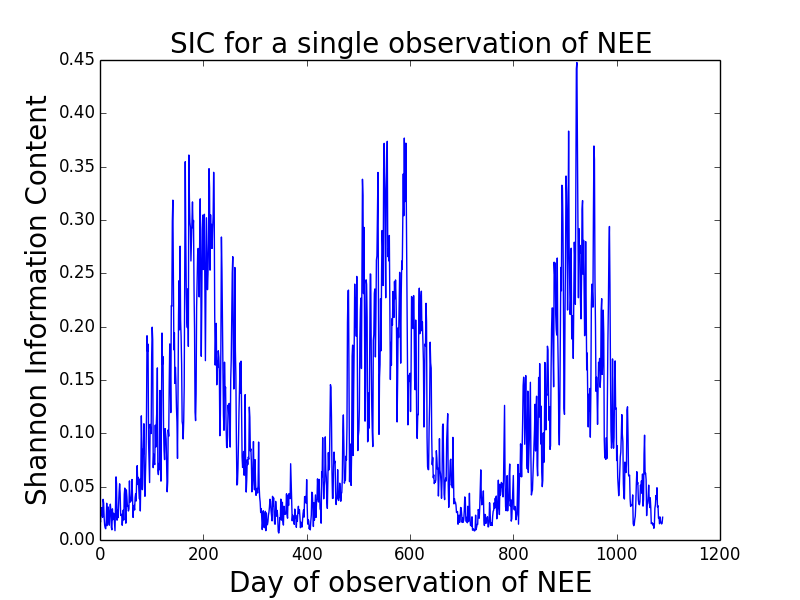
\includegraphics[width=.9\linewidth]{SIC1Obs_0_1095.png}
  \caption{$SIC$ for a single observation of $NEE$.}
  \label{fig:sub1}
\end{subfigure}%
\begin{subfigure}{.5\textwidth}
  \centering
  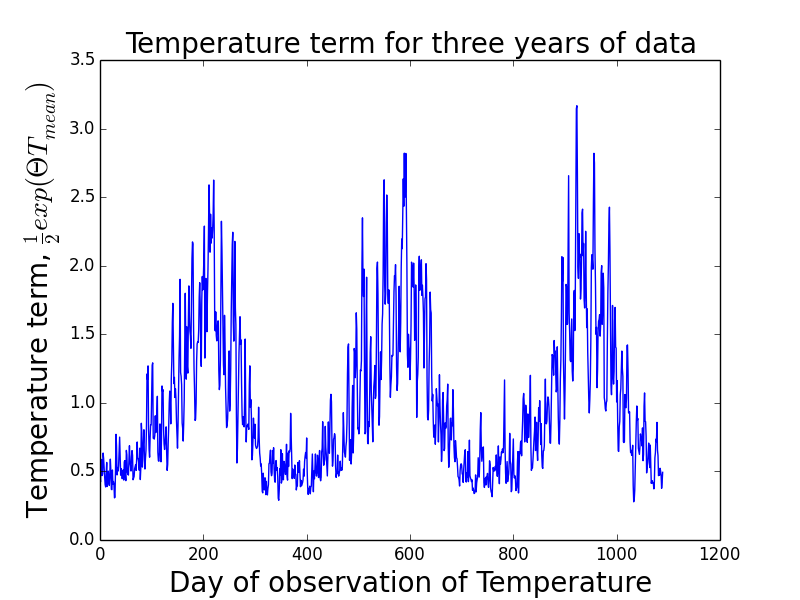
\includegraphics[width=.9\linewidth]{Temp_0_1095.png}
  \caption{Temperature term, $\frac{1}{2}exp(\Theta  T_{mean})$.}
  \label{fig:sub2}
\end{subfigure}
\caption{$SIC$ and temperature varying over three years using driving data from Oregon pine forest.}
\label{fig:SICNEET}
\end{figure}

However the relationship is not linear as the magnitude of $GPP$'s first derivative is also dependent on daily irradiance and the value of the foliar carbon pool ($C_f$). This shows that observations of $NEE$ made in the summer are much more valuable than those made in the winter assuming warmer temperatures, higher daily irradiance and a higher amount of foliar carbon in the summer. In the next section we consider a series of observations over some time window. We will see that it takes 14 observations of $NEE$ in winter to gain the same level of information as 1 observation of $NEE$ in the winter.

\subsection{$SIC$ for successive observations over a time window}%%%%%%%%%%%%%%%%%%%%%%

Following the results for $SIC$ based at a single time, we now consider the $SIC$ when successive observations are added over a period of time. The DALEC model is now built into a Four-Dimensional Variational Data Assimilation (4D-Var) framework where our observation operator, $\mathbf{H}$, and observation error covariance matrix, $\mathbf{R}$, are now,
\[ 
\mathbf{H}=
\begin{pmatrix}
\mathbf{H}_0 \\
\mathbf{H}_1\mathbf{M}_0\\
\vdots \\
\mathbf{H}_n\mathbf{M}_{n,0}
\end{pmatrix}
\hspace{5mm} \text{and} \hspace{5mm}
\mathbf{R}=
\begin{pmatrix}
\mathbf{R}_0 & 0 & 0 & 0 \\
0 & \mathbf{R}_1 & 0 & 0 \\
0 & 0 & \ddots & 0 \\
0 & 0 & 0 & \mathbf{R}_n
\end{pmatrix},
\]
where $\mathbf{H}_i$ is our linearized observation operator at time $t_i$, $\mathbf{M}_{i,0}=\mathbf{M}_{i-1}\mathbf{M}_{i-2}\cdots\mathbf{M}_0$ is our linearized model evolving the state vector, $\textbf{x}_b$, at time $t_0$ to time $t_i$ and $\mathbf{R}_i$ is the observation error covariance matrix corresponding to $\mathbf{H}_i$ at time $t_i$ \cite{lewis2006dynamic}. Firstly the tangent linear model for DALEC was calculated analytically as $\mathbf{M}_i=\frac{\delta \textbf{m}_i}{\delta \textbf{x}_i}$.

We begin by considering successive observations of $Cf$ in time. Here we again have,
\[
\mathbf{H}_{i} = \begin{pmatrix}
1 & 0 & 0 & 0 & 0
\end{pmatrix}
\hspace{5mm} \text{and} \hspace{5mm}
\mathbf{R}_i=\sigma_{cf,o}^{2}.
\] 
The linearized model at time $t_i$ is given as,
\[
\mathbf{M}_{i}=
\begin{pmatrix} 
(1-p_5)+p_3(1-p_2)GPP'(C_f(t_i),\phi) & 0 & 0 & 0 & 0 \\
p_4(1-p_3)(1-p_2)GPP'(C_f(t_i),\phi) & (1-p_7) & 0 & 0 & 0 \\
(1-p_4)(1-p_3)(1-p_2)GPP'(C_f(t_i),\phi) & 0 & (1-p_6) & 0 & 0 \\
p_5 & p_7 & 0 & (1-(p_1+p_8)T(t_i)) & 0 \\
0 & 0 & p_6 & p_1T(t_i) & (1-p_9T(t_i)) \\
\end{pmatrix}.
\]
Then for two successive observations of $Cf$ we have,
\[ 
\mathbf{H}=
\begin{pmatrix}
\mathbf{H}_0 \\
\mathbf{H}_1\mathbf{M}_0\\
\end{pmatrix}
=
\begin{pmatrix}
1 & 0 & 0 & 0 & 0 \\
(1-p_5)+p_3(1-p_2)GPP'(C_f(t_0),\phi) & 0 & 0 & 0 & 0\\
\end{pmatrix}
\]
and
\[
\mathbf{R}=
\begin{pmatrix}
\mathbf{R}_0 & 0  \\
0 & \mathbf{R}_1  \\
\end{pmatrix}
=
\begin{pmatrix}
\sigma_{cf,o}^{2} & 0  \\
0 & \sigma_{cf,o}^{2}  \\
\end{pmatrix}.
\]
We then have,
\[
SIC = \frac{1}{2}ln\begin{vmatrix} \mathbf{B} \end{vmatrix}\begin{vmatrix} \mathbf{J}'' \end{vmatrix} =\frac{1}{2}ln \bigg(1+\frac{\sigma_{cf,b}^{2}}{\sigma_{cf,o}^{2}}+\frac{\sigma_{cf,b}^{2}\eta_0^{2}}{\sigma_{cf,o}^{2}} \bigg),
\]
where $\eta_i=(1-p_5)+p_3(1-p_2)GPP'(C_f(t_i),\phi)$. We can continue adding more observations at successive times and we start to see a pattern. For three observations at successive times we have,
\[
SIC =\frac{1}{2}ln \bigg(1+\frac{\sigma_{cf,b}^{2}}{\sigma_{cf,o}^{2}}+\frac{\sigma_{cf,b}^{2}\eta_0^{2}}{\sigma_{cf,o}^{2}}+\frac{\sigma_{cf,b}^{2}\eta_0^{2}\eta_1^{2}}{\sigma_{cf,o}^{2}} \bigg),
\]
for four,
\[
SIC =\frac{1}{2}ln \bigg(1+\frac{\sigma_{cf,b}^{2}}{\sigma_{cf,o}^{2}}+\frac{\sigma_{cf,b}^{2}\eta_0^{2}}{\sigma_{cf,o}^{2}}+\frac{\sigma_{cf,b}^{2}\eta_0^{2}\eta_1^{2}}{\sigma_{cf,o}^{2}}+\frac{\sigma_{cf,b}^{2}\eta_0^{2}\eta_1^{2}\eta_2^{2}}{\sigma_{cf,o}^{2}} \bigg).
\]
Using a simple proof by induction we find that for $n$ observations we have,
\[
\text{$SIC$ for $n$ observations of $Cf$ }= \frac{1}{2}ln\bigg(1+\frac{\sigma_{cf,b}^{2}}{\sigma_{cf,o}^{2}}\big(1+\sum_{k=0}^{n-2}\prod_{i=0}^{k}\eta_i^{2}\big)\bigg)
\]
We have plotted the $SIC$ for increasing numbers of observations of $Cf$ using three years of meteorological driving data from an Oregan pine forest as seen in figure \ref{Cf_succ}.

\begin{figure}[h]
\centering
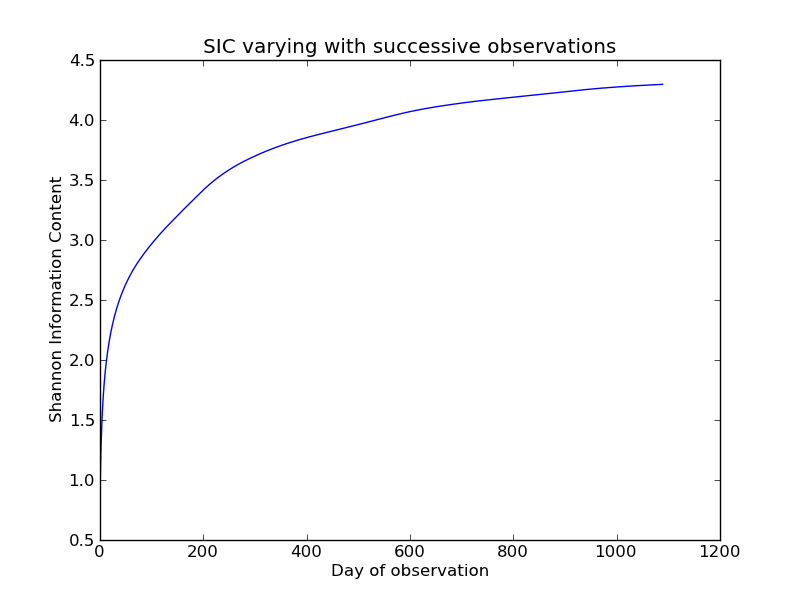
\includegraphics[width=.9\textwidth]{SIC_0_1090Cf.png}
\caption{$SIC$ varying as successive observations of $Cf$ are added using driving data from Oregon pine forest.}
\label{Cf_succ}
\end{figure}

As before with a single observation at one time we can repeat this with successive observations of $NEE$ instead of $Cf$ this is plotted in figure \ref{SIC_succ}. Here we can see the seasonal cycle of information content as in figure \ref{fig:SICNEET} with little information being added during the winter months and more being added during summer.

\begin{figure}[ht]
\centering
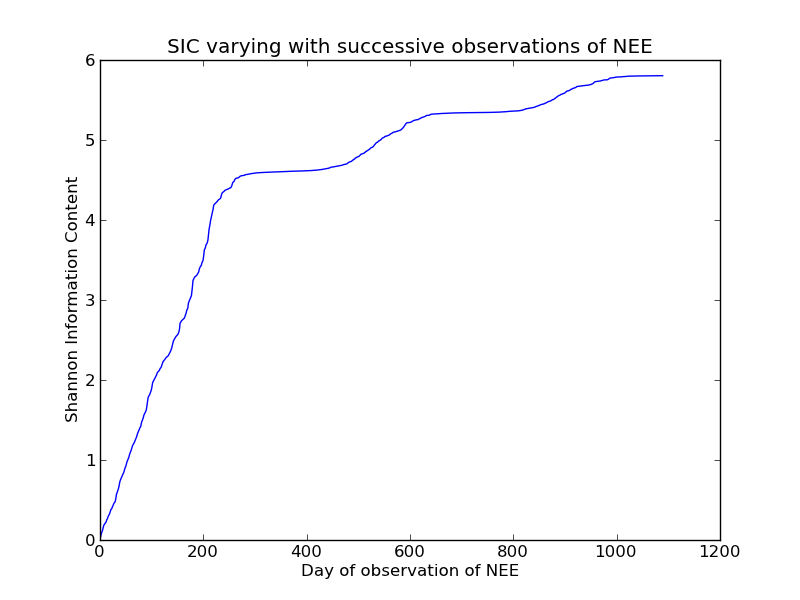
\includegraphics[width=.9\textwidth]{SIC_0_1090.png}
\caption{$SIC$ varying as successive observations of $NEE$ are added using driving data from Oregon pine forest.}
\label{SIC_succ}
\end{figure} 



%\begin{figure}[h]
%\centering
%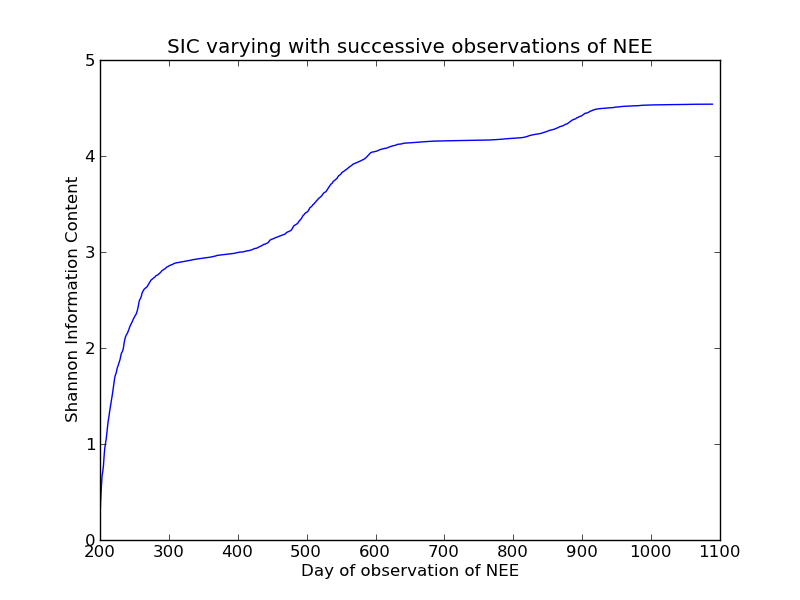
\includegraphics[width=.9\textwidth]{SIC_200_1090.png}
%\caption{$SIC$ varying as successive observations of $NEE$ are added using driving data from Oregon pine forest. Starting at day %200.}
%\label{fig:SIC_subplot}
%\end{figure}

%\begin{figure}[h]
%\centering
%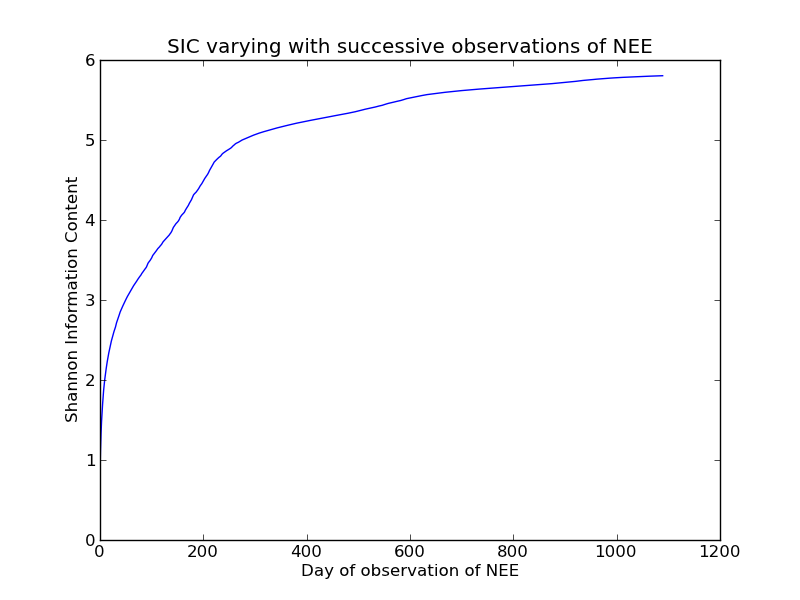
\includegraphics[width=.9\textwidth]{SIC_0_1090CfNEE.png}
%\caption{$SIC$ varying as successive observations of $NEE$ and $Cf$ are added using driving data from Oregon pine forest.}
%\label{fig:SIC_subplot}
%\end{figure}

\section{Degrees of freedom for signal for DALEC}%%%%%%%%%%%%%%%%%%%%%%


\begin{figure}[h]
\centering
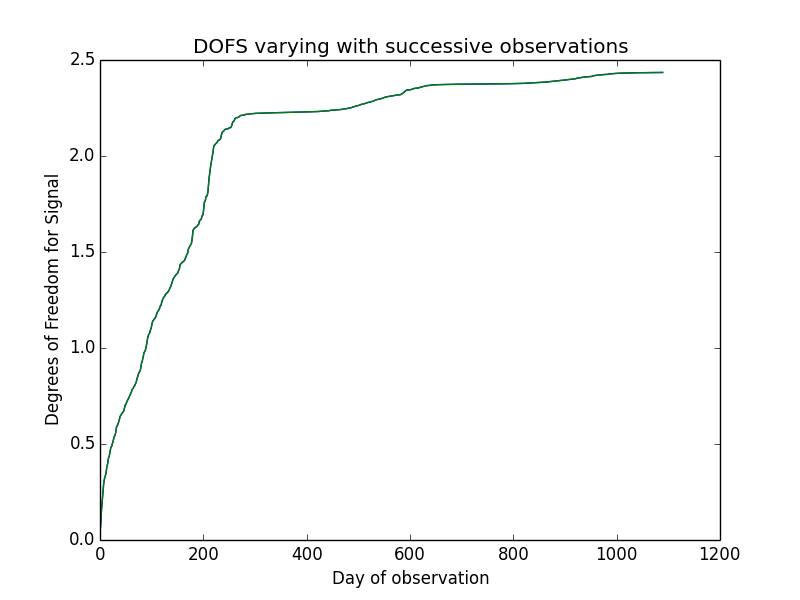
\includegraphics[width=.9\textwidth]{DOFS_0_1090Cf_Cpoolsconst.png}
\caption{$DOFS$ varying as successive observations of $NEE$ are added using driving data from Oregon pine forest.}
\label{fig:SIC_subplot}
\end{figure}

\section{Conclusion}%%%%%%%%%%%%%%%%%%%%%%

\bibliography{../PhD}{}
\bibliographystyle{plain}
\end{document}
